\documentclass[a4paper,14pt]{extreport}

\usepackage[T1,T2A]{fontenc}
\usepackage[utf8]{inputenc}

\usepackage{style/bsumain}
\usepackage{style/bsudiplomatitle14}
\usepackage{blindtext}
\usepackage{float}

\subfaculty{Кафедра биомедицинской информатики}
\title{Изучение методов описания химических соединений для примемения в алгоритмах машинного обучения}
\author{Малыщика Акима Андреевича\\
студента 3 курса 3 группы\\
специальность "информатика"}
\mentor{профессор кафедры БМИ\\
Тузиков Александр Васильевич
        }
\reviewer{Орлович Юрий Леонидович \\
          заведующий каведры БМИ}

\usepackage{graphicx}
\begin{document}
\maketitle
\setcounter{page}{2}
\begin{center}
  \large\bfseries{РЕФЕРАТ}
\end{center}

Курсовой проект, 20 стр., 5 иллюстр., 9 источников.

\textbf{Ключевые слова:} ДЕСКРИПТОРЫ, МОЛЕКУЛЯРНЫЕ ФИНГЕРПРИНТЫ, SMILES.

\textbf{Объекты исследования --} дескрипторы химических соединений, алгоритмы машинного обучения на основе дескрипторов.

\textbf{Цель исследования --} изучение существующих молекулярных дескрипторов и алгоритмов на их основе.

\textbf{Методы исследования --} системный подход, изучение соответствующей литературы и электронных источников.

\textbf{В результате исследования} изучены графовые структуры, молекулярные фингерпринты и SMILES, исследованы алгоритмы обработки дескрипторов, рассмотрены архитектуры нейросетей на основе SMILES-описаний.

\textbf{Области применения --} хемоинформатика, медицина, фармацевтика.

\newpage
  {
    \renewcommand{\contentsname}{Содержание}
    
    \tableofcontents
  }

  \chapter*{Введение}
  \addcontentsline{toc}{chapter}{Введение}
  \label{c:introduction}

Компьютерное моделирование лекарств — относительно быстро развивающаяся и достаточно перспективная отрасль IT-индустрии, в которой активно используются алгоритмы машинного обучения. Генеративные нейронные сети применяются для получения новых соединений, которые потенциально могут стать основой для лекарственных средств. Основная проблема такого подхода в том, что на данный момент не существует универсального метода кодирования химических соединений, который был бы лучше всех остальных в любой ситуации. Таким образом, задачи данного курсового проекта:

\begin{enumerate}
\item Изучить существующие на данный момент методы описания (дескрипторы) химических соединений
\item Исследовать их преимущества и недостатки
\item Рассмотреть алгоритмы генерации молекул на основе существующих дескрипторов.
\end{enumerate}

Цель проекта -- сбор теоретической базы для дальнейших исследований. В дальнейшем работу над проектом можно будет продолжить, проведя сравнительный анализ дескрипторов на конкретной мишени, и сделать выводы касательно наиболее удачного способа описания молекул веществ в конкретной ситуации.

Способов описать химическое соединение существует достаточно много. В рамках данного проекта все они рассмотрены не будут, предпочтение будет отдано тем методам, которые потенциально перспективны для использования в области машинного обучения.
Основные способы представить химическое соединение в памяти компьютера:
\begin{enumerate}
  \item Графы структур соединений
  \item Бинарные векторы свойств (молекулярные фингерпринты)
  \item Линейные представления (SMILES, IChI)
\end{enumerate}

В данном проекте рассмотрены перечисленные методы, изучены их преимущества и недостатки, а также исследованы области их применения.

  
  
  
  

  
  
  \chapter{Графы структур}
  \label{c:graphs}
  
  С точки зрения математики, графом $G(V,E)$ называется совокупность непустого множества $V$ и множества $E$ неупорядоченных пар различных элементов множества $V$. Множество $V$ называется ''множеством вершин'', множество $E$ называется ''множеством рёбер''.

$$G(V,E) = \left \langle V,E \right \rangle, \quad  V  \ne \varnothing , \quad E \subseteq V \times V , \quad  \left \{ v,v \right \} \notin E, \quad v \in V .$$
  
  Поскольку молекулы состоят из атомов и связей между ними, идея представить химическое соединение в виде графа его структуры кажется вполне естественной. Существует несколько способов представления графов в памяти компьютера:
  \begin{enumerate}
	\item Матрица смежности
	\item Матрица расстояний
	\item Матрица инцидентности
	\item Матрица связей
\end{enumerate}
Рассмотрим каждый из них.
  
  

  \section{Матрица смежности}
  \label{s:matrix_1_sec}
  При таком способе хранения соединения заводится матрица размера N*N, где N — число атомов в соединении. Матрица заполняется нулями, если связь между атомами отсутствует и единицами, если связь есть. Поскольку матрица смежности симметрична, расход памяти, занимаемой матрицой, можно уменьшить, если хранить только её треугольную форму. Также для большей эффективности представления и экономии памяти из соединения можно исключить связи с атомами водорода, ведь их можно будет при необходимости восстановить по правилам валентности. Недостатком матрицы смежности является то, что в ней не содержится информации о типах связей между атомами в молекуле. Таким образом, информация, которую содержит такая матрица, позволяет построить граф молекулы, однако по ней невозможно восстановить полную структуру соединения.
  \section{Матрица расстояний}
  \label{s:matrix_2_sec}
  Матрица расстояний, как и матрица смежности, симметрична, и её размер (NxN) также зависит только от числа атомов в соединении. Матрица содержит расстояния между соответствующими атомами в молекуле. К матрице расстояний применимы те же оптимизации по расходу памяти, что и к матрице смежности.
  
  Расстояния между атомами можно задавать двумя способами. Первый — с помощью евклидовой метрики:
  $$d(a,b)=\sqrt{(a_1-b_1)^2+(a_2-b_2)^2+(a_3-b_3)^2}.$$
  В таком случае расстояния выражаются в ангстремах или нанометрах. Второй способ — топологическое расстояние (минимальное количество связей в графе соединения между атомами A и B). 
  
  Таким образом, матрицы расстояний имеют те же проблемы, что и матрицы смежности: информации в них недостаточно для полного восстановления структуры соединения. Однако, они позволяют воссоздать расположение атомов в трёхмерном пространстве.


  \section{Матрица инцидентности}
  \label{s:matrix_3_sec}
  Матрица инцидентности, в отличие от остальных матриц, представляет собой прямоугольную матрицу MxN, её размеры зависят от числа атомов и числа связей в молекуле. Как и матрица смежности, матрица инцидентности показывает лишь наличие либо отсутствие какой-либо связи, без указания её типа. Размеры матрицы инцидентности можно уменьшить, если не рассматривать атомы водорода.

  \section{Матрица связей}
  \label{s:matrix_4_sec}
  Матрица связей решает проблему всех рассмотренных выше матриц. Как и матрица смежности, она представляет собой квадратную матрицу NxN. Но эта матрица не является бинарной, она хранит порядки связей между атомами, а не только нули и единицы. Порядок связи для несвязанных между собой атомов формально полагается равным 0. Соответственно, двойная связь обозначается числом 2, тройная — числом 3, и т.д.

К матрице связей можно применить те же методы сокращения расхода памяти, что и к матрице смежности (удаление атомов водорода, симметричной части). Данная матрица содержит достаточно информации для полного восстановления структуры соединения. Однако, в случае наличия в соединении ароматических связей, для которых нет конкретного значения порядка связи, представление молекулы с помощью данной матрицы будет неоднозначным, и необходимы дополнительные соглашения касательно того, как обозначать такие связи.
\begin{figure}[htp]
\centering
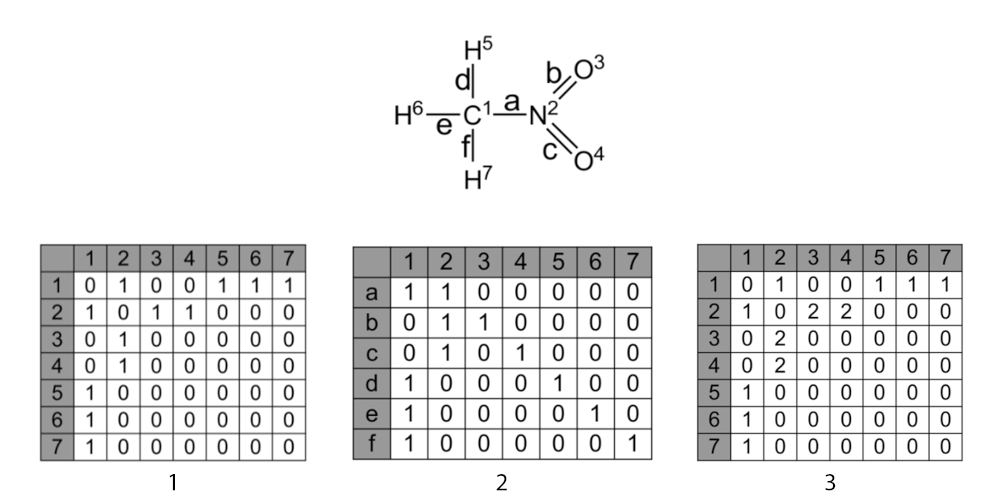
\includegraphics[scale=0.35]{images/нитрометан.png}
\caption{Представление молекулы нитрометана \\матрицей смежности (1), матрицей инцидентности (2), матрицей связей (3)}
\label{nitromethane}
\end{figure}

  \section{Применение графов соединений в машинном обучении}
  \label{s:graphs_applications}
Графовые структуры данных могут быть полезными для предварительной обработки данных о соединениях, закодированных другими способами. К примеру, особенностью SMILES-описаний химических соединений является их неуникальность. Чтобы избежать проблемы дублирования соединений, сгенерированные нейросетью SMILES-молекулы можно канонизировать, после чего удалить явные дубликаты. Впоследствии это позволит ускорить процедуру докинга, поскольку провести его будет нужно для меньшего числа соединений. Алгоритм канонизации SMILES-описаний основан на алгоритме канонизации графа, то есть для его работы необходимо преобразовать соединение из SMILES в какое-нибудь из матричных представлений, и произвести процедуру канонизации помеченного графа.

Тем не менее, разрабатывать нейронные сети на основе графов соединений практического смысла не имеет. Во-первых, большинство матричных структур не позволяет хранить достаточно информации о свойствах соединения, а значит, нейросеть не сможет выявить закономерности, необходимые для генерации соединений с аналогичными свойствами. Во-вторых, из матричного представления не всегда возможно однозначно восстановить закодированное соединение, что делает мало полезным генерацию веществ в таком виде и заставляет задуматься о применении других способов описания молекул.


  \chapter{Молекулярные фингерпринты}
  \label{c:fingerprints}
  Молекулярные фингерпринты – достаточно известный способ векторизации молекулярных данных, он часто используется при обучении с учителем, а также для поиска соединений со схожими свойствами.
  
Молекулярные фингерпринты — это битовые строки, в которых каждый бит отвечает за наличие или отсутствия какого-либо фрагмента в соединении. При этом не существует универсальных меток для каждого бита. Молекулярный фингерпринт, как правило, генерируется из самой молекулы. 

  \section{Алгоритм генерации фингерпринтов}
  \label{s:fp_generation_sec}
  Алгоритов генерации молекулярных опечатков существует несколько. Рассмотрим алгоритм, используемый компанией Daylight. Этот алгоритм исследует молекулу и генерирует признаки для следующих паттернов (подструктур):
  \begin{itemize}
	\item паттерн для каждого атома
	\item паттерн, представляющий каждый атом и его ближайших соседей (а также связи между ними)
	\item паттерн, представляющий каждую группу атомов, соединённых путями длиной до 2 связей
	\item паттерн, представляющий каждую группу атомов, соединённых путями длиной до 3 связей
	\item и т.д.
  \end{itemize}
К примеру, для молекулы $\bold{OC=CN}$ алгоритм бы сгенерировал следующие паттерны:

\begin{table}[H]
\caption{Список сгенерированных паттернов}
\begin{center}
\begin{tabular}{cccc}
	Длина пути 0: & C & O & N\\
	Длина пути 1: & OC & C=C & CN\\
	Длина пути 2: & OC=C & C=CN\\
	Длина пути 3: & OC=CN
\end{tabular}
\end{center}
\end{table}


Список полученных паттернов исчерпывающий: таблица содержит все подструктуры исходной молекулы. Очевидно, на практике количество паттернов, необходимых для описания больших соединений может быть просто огромным. При этом, чтобы производить какие-либо операции над фингерпринтами, требуется фиксированная длина отпечатка для всех молекул в датасете. Но тогда, если использовать вектор слишком большой длины для маленьких соединений, большая часть вектора будет заполнена нулями. И наоборот, при использовании слишком маленьких фингерпринтов для больших соединений весь фингерпринт будет заполнен единицами (и, возможно, будет при этом хранить не всю информацию о соединении). Чтобы избавиться от этих проблем, фингерпринты подвергают процедуре фолдинга.


  \section{Фолдинг фингерпринтов}
  \label{s:fp_folding_sec}
 Процесс фолдинга начинается с фиксированного размера фингерпринта, достаточно большого для полного представления структуры молекулы. Далее фингерпринт сворачивается (англ. fold): происходит его разделение на две части, которые складываются при помощи логического оператора OR. На выходе получается более короткий фингерпринт с более высокой плотностью информации на бит. Процесс фолдинга можно повторить несколько раз, пока не будет достигнута желаемая плотность информации.
 
Однако, таким образом может быть потеряна часть информации. Рассмотрим фингерпринты подструктуры P и молекулы M. Если все биты подструктуры P изначально находятся в молекуле M, то это будет справедливо и после фолдинга. С другой стороны, если хотя бы один бит из P изначально не в M, то после фолдинга может оказаться, что подструктура P содержится в M. Это может привести к тому, что при виртуальном скрининге найдётся больше соединений с подструктурой P, чем нужно. С каждой процедурой фолдинга будет увеличиваться вероятность найти ''лишние'' молекулы, однако фингерпринт будет занимать в два раза меньше пространства.

Таким образом, генерировать фингерпринты фиксированной длины необязательно, достаточно сгенерировать фингерпринт любой длины, представляющий полную структуру соединения, и с помощью фолдинга привести его к необходимому фиксированному размеру. 
 
  
  \section{Сравнение фингерпринтов}
  \label{s:fp_comparing_sec}
Для сравнения двух молекулярных отпечатков соединений достаточно сравнить их побитово. Рассмотрим фингерпринты A и B. При их сравнении возможны 4 ситуации, представленные в таблице 2.2.
  
\begin{table}[H]
\caption{Побитовое сравнение фингерпринтов A и B}
\begin{center}
\begin{tabular}{|c|c|c|c|}
\hline
	& 0 & 1 & Сумма\\
\hline
	0 & d & b & b + d\\
\hline
	1 & a & c & a + c\\
\hline
	Сумма & a + d& b + c & n\\
\hline
\end{tabular}

\end{center}
где:
\begin{itemize}
\item a – количество битов, равных единице в фингерпринте А и нулю в B.

\item b – количество битов, равных единице в фингерпринте B и нулю в A.

\item c – количество битов, равных единице в обоих фингерпринтах.

\item d – количество битов, равных нулю в обоих фингерпринтах.
\end{itemize}
\end{table}
На основе данных показателей существует множество метрик для сравнения двух соединений. Некоторые из них представлены в таблице 2.3.
\begin{table}[H]
\caption{Метрики для сравнения фингерпринтов}
\begin{center}
\begin{tabular}{|c|c|c|}
\hline
	Метрика & Область значений & Формула\\[2ex]
\hline
	Дайс & $[0, 1]$ & $\frac{2c}{(a+c)+(b+c)}$\\[5ex]
\hline
	Евклид & $[0, 1]$ & $\sqrt{\frac{c + d}{a + b + c + d}}$\\[5ex]
\hline
	Манхэттен & $[1, 0]$ & $\frac{a + b}{a + b + c + d}$\\[5ex]
\hline
	Танимото & $[0, 1]$ & $\frac{c}{a + b + c}$\\[5ex]
\hline
	Симпсон & $[0, 1]$ & $\frac{c}{min((a+c),(b+c))}$\\[5ex]
\hline
\end{tabular}
\end{center}
\end{table}
\newpage
\begin{lstlisting}[language=Python, caption=Использование метрики Дайса и библиотеки RDKit для сравнения двух фингерпринтов Моргана]
>>> from rdkit.Chem import MolFromSmiles
>>> from rdkit.Chem.AllChem import GetMorganFingerprint
>>> from rdkit.DataStructs import DiceSimilarity
>>> molecule_1 = MolFromSmiles('Cc1ccccc1')
>>> molecule_2 = MolFromSmiles('Cc1ncccc1')
>>> fingerpint_1 = GetMorganFingerprint(molecule_1, 2)
>>> fingerpint_2 = GetMorganFingerprint(molecule_2, 2)
>>> DiceSimilarity(fingerpint_1,fingerpint_2)
0.55...
\end{lstlisting}


  \section{Распространённые виды фингерпринтов}
  \label{s:fp_types_sec}

  \subsection{Фингерпринты Моргана}
  \label{ss:fp_morgan_subsec}
  Моргановские фингерпринты – это 2048-битные векторы, названные в честь ученого, который предложил алгоритм их генерации. Алгоритм Моргана генерации молекулярных фингерпринтов работает следующим образом:
Для каждого атома в соединении вычисляются следующие показатели:
\begin{enumerate}
\item количество ближайших соседей (кроме атомов водорода)
\item количество связей у атома (без учета связей с атомами водорода)
\item атомный номер
\item атомная масса
\item количество связей с атомами водорода
\item принадлежит атом циклу (1) или нет (0)?
\end{enumerate}
Данные показатели хэшируются. Таким образом у каждого атома появляется его идентификатор (хэш-значение). Первая итерация завершена. 

Далее для каждого атома заводится массив его соседей и связей между ними, отсортированный по хэш-значениям атомов. Этот массив также хэшируется, а полученное значение становится новым идентификатором атома. Таким образом, на первой итерации алгоритма произойдёт хэширование отдельных атомов, на второй – хэширование атомов с их соседями диаметра 1, на третьей – с соседями диаметра 2 и т.д. После завершения итерационного процесса производят конкатенацию хэш-значений всех атомов, и с помощью фолдинга полученный вектор переводят в бинарный вектор длины 2048 бит.

  \subsection{Структурные ключи MACCS}
  \label{ss:fp_maccs_subsec}
  Структурные ключи отличаются от обычных фингерпринтов тем, что в них заранее определено, за что отвечает каждый бит. Ключи MACCS (Molecular ACCess System), также известные как ключи MDL, названы так в честь разработавшей их компании. Существует две разновидности ключей MACCS (одна содержит 960 ключей, другая – её подмножество из 166 ключей). Краткое описание каждого из ключей можно найти в репозитории компании.

  \subsection{Другие виды фингерпринтов}
  \label{ss:fp_other_subsec}
  Помимо двух вышеописанных, существуют, например, фингерпринты PubChem (длины 881 бит, применяются для поиска по одноименной базе данных). Также иногда имеет смысл заменить хэш-функции в алгоритме создания фингерпринта на дифференцируемые функции, что позволит “обучать” фингерпринт вместе с нейросетью, оптимизируя таким образом фингерпринт под конкретную задачу и достигая больших успехов, чем при работе со стандартными фингерпринтами [\ref{itm:lit7}].
  
  \section{Применение фингерпринтов в машинном обучении}
  \label{s:fp_application}
  Молекулярные фингерпринты получили широкое применение в машинном обучении. На их основе создают модели для предсказания токсичности молекул [\ref{itm:toxic}], растворимости веществ [\ref{itm:lit7}], и прочих показателей, расчет которых экспериментальным путем потребовал бы гораздо больших финансовых затрат.
  
Тем не менее, молекулярные фингерпринты имеют один большой недостаток: простого универсального метода восстановления изначальной структуры соединения, которое представлено в виде фингерпринта, не существует. А восстановление структуры оказывается особенно важным при работе с соединениями, которые сгенерированы с помощью искусственного интеллекта, и которые при этом необязательно могут быть найдены в базах данных существующих молекул.
Этого недостатка лишены линейные методы представления соединений, такие как SMILES-описания.

  
  \chapter{SMILES}
  \label{c:smiles}
  SMILES (Simplified Molecular Input Line Entry System) — линейная нотация для ввода и представления молекул и реакций. SMILES содержит ту же информацию, что и расширенные матрицы связей. Основная причина, по которой SMILES полезнее матрицы связей, в том, что SMILES скорее языковая структура, чем структура данных. При этом алфавит и количество правил SMILES-кодирования невелико, что позволяет, во-первых, легко кодировать и декодировать соединения вручную, а во-вторых, позволяет без проблем применять к SMILES те же методы машинного обучения, что и к естественным языкам.
Еще одним преимуществом языка SMILES является компактность записи соединений с его помощью (относительно других линейных нотаций и прочих методов описания соединений).

\begin{table}[H]
\caption{Сравнение представлений SMILES и InChI}
\begin{center}
\begin{tabular}{|l|l|l|l|}
\hline
	Формула & Код SMILES & Код InChI\\
\hline
	$CH_3CH_2OH$ & CCO & InChI=1S/C2H60/c1-2-3/h3H,2H2,1H3\\
\hline
	$CH_3CH=O$ & CC=O & InChI=1S/C2H4O/c1-2-3/h2H,1H3\\
\hline
	$CH_3COOH$ & CC(O)=O & InChI=1S/C2H4O2/c1-2(3)4/h1H3,(H,3,4)\\
\hline
\end{tabular}
\end{center}
\end{table}


Из таблицы видно, что для кодирования с помощью SMILES, как правило, требуется в разы меньше символов, чем для кодирования с помощью международного химического идентификатора InChI. Также соединения в виде SMILES занимают в памяти компьютера на 50-70\% меньше пространства, чем те же соединения, представленные в виде матриц связей их атомов.

  \section{Правила кодирования SMILES}
  \label{s:smiles_coding_sec}
  SMILES нотация представляет собой не разделенную пробелами последовательность символов. Запись SMILES получается в результате обхода в глубину вершин молекулярного графа.
Как правило, SMILES не включает в себя атомы водорода (связи C-H, N-H, O-H, S-H), поскольку их можно восстановить по правилам валентности.
\newpage
\begin{table}[H]
\caption{Примеры молекул без атомов водорода в SMILES}
\begin{center}
\begin{tabular}{|c|c|c|}
\hline
	C & метан & $CH_4$\\
\hline
	P & фосфин & $PH_3$\\
\hline
	N & аммиак & $NH_3$\\
\hline
	S & сероводород & $H_2S$\\
\hline
	O & вода & $H_2O$\\
\hline
	Cl & соляная кислота & $HCl$\\
\hline
\end{tabular}
\end{center}
\end{table}

Циклы в графах соединений разъединяются, места разъединения обозначаются числами, показывающими наличие связей в исходной структуре соединения.

\begin{figure}[htp]
\centering
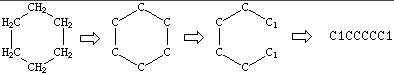
\includegraphics[scale=1.20]{images/Screenshot from 2021-12-04 16-34-09.png}
\caption{Разъединение циклов в SMILES}
\label{cycles}
\end{figure}

Точки ветвления обозначаются круглыми скобками.

\begin{figure}[htp]
\centering
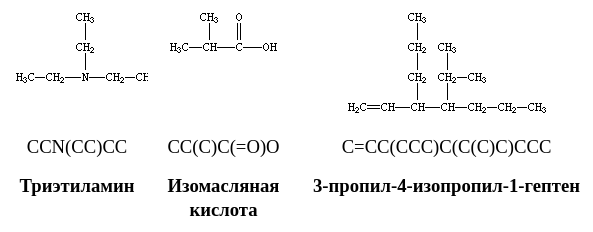
\includegraphics[scale=0.80]{images/Screenshot from 2021-12-04 16-45-58.png}
\caption{Примеры соединений с точками ветвления}
\label{branches}
\end{figure}

Двойную связь обозначают символом =, тройную – символом \#.

\begin{table}[H]
\caption{Примеры соединений с двойными и тройными связями}
\begin{center}
\begin{tabular}{|l|c|c|}
\hline
	C=O & Формальдегид & $CH_2O$\\
\hline
	C=C & Этен & $CH_2=CH_2$\\
\hline
	O=C=O & Углекислый газ & $CO_2$\\
\hline
	C\#N & Цианид & $HCN$\\
\hline
\end{tabular}
\end{center}
\end{table}

Для обозначения конфигурации асимметрического тетраэдрического атома углерода используются символы @ (против часовой стрелки) и @@ (по часовой стрелке). Для обозначения конфигурации следует смотреть на хиральный центр со стороны заместителя, стоящего в строке SMILES перед этим центром. В полном соответствии с последовательностью в строке SMILES трёх других заместителей определяется часовое направление, которое указывается как @ или @@ возле асимметрического атома углерода, заключаемого в квадратные скобки.

Атом водорода в конфигурационных кодах указывается обязательно и, если помещается в строке SMILES сразу после хирального центра, то может вместе с ним заключаться в квадратные скобки.


\begin{figure}[htp]
\centering
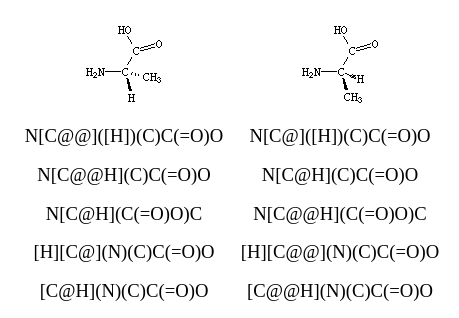
\includegraphics[scale=0.80]{images/Screenshot from 2021-12-04 16-57-53.png}
\caption{Разные конфигурации одних и тех же структур}
\label{configs}
\end{figure}

Символами $/\ \backslash$ обозначается конфигурация относительно двойной связи.

\begin{figure}[htp]
\centering
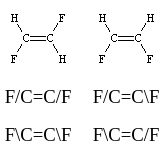
\includegraphics[scale=1.00]{images/Screenshot from 2021-12-04 16-59-41.png}
\caption{Примеры кодирования цис- и транс- изомеров}
\label{isomeric}
\end{figure}


\begin{table}[H]
Изотопы обозначаются числами перед атомами.
\caption{Примеры кодирования изомеров в SMILES}
\begin{center}
\begin{tabular}{|c|c|}
\hline
	Код SMILES &  Название\\
\hline
	[12C] & Углерод-12\\
\hline
	[13C] & Углерод-13\\
\hline
	[13CH4] & С-13 метан\\
\hline
\end{tabular}
\end{center}
\end{table}

Ионизация обозначается символами + и - с указанием числа ионов, если оно не равно единице.

\begin{table}[H]
\caption{Примеры кодирования катионов и анионов в SMILES}
\begin{center}
\begin{tabular}{|l|l|}
\hline
	[H+] & протон\\
\hline
	[Fe++2] & катион железа (II)\\
\hline
	[OH-] & гидроксильный анион\\
\hline
	[Fe++] & катион железа (II)\\
\hline
	[NH4+] & катион аммония\\
\hline
\end{tabular}
\end{center}
\end{table}

  \section{Применение SMILES в машинном обучении}
  \label{s:smiles_application}
  Как уже было отмечено, использование представления химических соединений с помощью языка SMILES позволяет применять к соединениям те же подходы, что и, например, при работе с текстовой информацией. Это значит, что для генерации соединений подойдут те же архитектуры нейронных сетей, что и для генерации текстов. На данный момент существует множество генераторов соединений, основанных на рекуррентных нейронных сетях и LSTM (Long Short Term Memory), а также на автоэнкодерах и гетероэнкодерах.
  \subsection{Предварительная обработка SMILES-датасета}
  \label{ss:smiles_preprocessing_subsec}
  В ходе проведённых исследований [\ref{itm:lit4}] было выяснено, что из входных данных имеет смысл исключать следующие соединения:
  \begin{enumerate}
  \item Не валидные SMILES-представления
  \item Соединения без атомов углерода
  \item Соединения с атомами, не входящими в состав потенциальных лекарств (отличными от H, C, N, O, P, S, F, Cl, Br, I)
  \item Соединения длиной более 120 символов
  \item Соединения с молекулярной массой > 1000 а.е.м.

  \end{enumerate}
  
    После фильтрации имеет смысл избавиться от дубликатов по названиям соединений, а также по SMILES (можно удалить как явные дубликаты, так и сравнить канонические SMILES-представления и удалить совпадающие).
    
   Далее закодированные в SMILES соединения с помощью one-hot кодирования переводят в бинарные вектора размера (максимальная длина SMILES)x(количество уникальных символов в SMILES), после чего датасет можно использовать для обучения моделей нейронных сетей.
  
  \subsection{Архитектуры нейросетей на основе SMILES}
  \label{ss:fp_other_subsec}
  Ещё одним преимуществом SMILES по сравнению с фингерпринтами является то, что SMILES представления последовательны. В отличие от фингерпринтов, которые содержат информацию об отдельных фрагментах структуры молекулы, SMILES описания позволяют анализировать всю структуру целиком. Последовательность SMILES делает возможным использовать данные представления в рекуррентных нейронных сетях в целом и в LSTM-сетях в частности. LSTM-слои позволяют нейросетям находить закономерности в SMILES-представлениях в контексте всей их структуры, а не только отдельно взятых её фрагментов.
  
  Другой перспективной архитектурой для генерации SMILES-описаний являются автокодировщики (англ. autoencoders). Составными частями данной архитектуры являются кодировщик (энкодер) и декодировщик (декодер). Энкодер сжимает входные данные и добавлет к ним случайный шум. Декодер отвечает за генерацию новых соединений путём восстановления их из сжатых энкодером данных. При реализации кодировщиков используют, в том числе, упомянутые LSTM-слои. Автоэнкодеры можно использовать как для обучения без учителя, так и для обучения с частичным подключением учителя (к примеру, в скрытое пространство сети можно добавить нейрон с желаемой энергей связи, не связанный с кодировщиком, что позволит получить на выходе соединения с заданным свойством [\ref{itm:lit4}]).
  
  Дальнейшей идеей развития архитектуры автоэнкодеров являются гетероэнкодеры. Данная архитектура содержит в себе несколько энкодеров и декодеров, что позволяет, во-первых, оптимизировать вычисления (можно использовать относительно простые энкодеры и декодеры), а, во-вторых, получать на выходе соединения разных типов (каждый декодер будет генерировать соединения своим особым образом). К примеру, можно воспользоваться неуникальностью SMILES представлений, и в качестве входных данных в разные энкодеры подать все возможные SMILES-представления одного и того же соединения [\ref{itm:lit9}]. Тогда на выходе из разных декодеров можно будет получить разные представления одного и того же соединения (при идеальных кодировщике и декодировщике), либо несколько соединений с похожими структурой и свойствами.
  
  Таким образом, многие архитектуры нейронных сетей, подходящие для работы с естественными языками, можно успешно применять и для генерации потенциальных лекарственных соединений.
  

  \chapter*{Заключение}
  \addcontentsline{toc}{chapter}{Заключение}
  \label{c:conclusion}
 В ходе проекта были:
  \begin{enumerate}
  \item Исследованы такие методы описания химических соединений, как графы, фингерпринты и SMILES
  \item Изучены алгоритмы для работы с данными методами (канонизация, фолдинг и др.)
  \item Рассмотрены архитектуры нейронных сетей, в которых применимы данные методы
  \item Изучены варианты предварительной обработки SMILES-датасета
  \item Изучена библиотека RDKit.
  \end{enumerate}
  

  \chapter*{Список использованных источников}
  \addcontentsline{toc}{chapter}{Список использованных источников}
  \label{c:literature}
\begin{enumerate}
\item \label{itm:lit1} Введение в хемоинформатику: Компьютерное представление химических структур: учеб. пособие / Т.И. Маджидов, И.И. Баскин, И.С. Антипин, А.А. Варнек. – Казань, Москва, Страсбург, 2020 – 176 с.
\item \label{itm:lit2} Чумаков А.А., Слижов Ю.Г. Система SMILES-кодирования молекулярных структур и её применение для решения научно-исследовательских задач. Национальный исследовательский Томский государственный университет, Электронное методическое пособие, 2017.–18 с.
    
    \item \label{itm:lit4} M.A. Shuldau et al. Development of molecular autoencoders as generators of protein inhibitors:
Application for prediction of potential drugs against coronavirus SARS-CoV-2 //Proceedings of
the 15th Ibterbational Conference on Pattern Recognition and Information Processing
(PRIP’2021), Sep. 21-24, 2021, Minsk, Belarus, 2021.
	\item \label{itm:lit5} Fingerprints – Screening and Similarity. – 2019. – 1 c. – URL: https://www.daylight.com/dayhtml/doc/theory/theory.finger.html  (дата обращения: 24.10.2021, 18:31)
	\item \label{itm:lit6} A Practical Introduction to the Use of Molecular Fingerprints in Drug Discovery. – 2019. – 1 c. – URL: https://towardsdatascience.com/a-practical-introduction-to-the-use-of-molecular-fingerprints-in-drug-discovery-7f15021be2b1 (дата обращения: 02.11.2021, 15:28)
	
	\item \label{itm:toxic} Mayr A. et al. DeepTox: toxicity prediction using deep learning //Frontiers in Environmental Science. – 2016. – 80 c.
	
	\item \label{itm:lit7} Convolutional Networks on Graphs for Learning Molecular Fingerprints / David Duvenaud [и др.] // Harvard University, 2015 – 9 c.
	\item \label{itm:lit8} SMILES – A Simplified Chemical Language. – 2019. – 1 c. – URL: https://www.daylight.com/dayhtml/doc/theory/theory.smiles.html (дата обращения: 15.11.2021, 22:03)

	\item \label{itm:lit9} Bjerrum, E.J.; Sattarov, B. Improving Chemical Autoencoder Latent Space and Molecular De Novo Generation Diversity with Heteroencoders. – 2018. 131 c. https://doi.org/10.3390/biom8040131 
    

\end{enumerate}
\end{document}
